% !TX root = Simulation.tex

\chapter{Fractals - Text Chapter 7}

\section{Problem 10}
\textbf{ Implement a bracketed OL-system and reproduce all plant-like structures of Figure 7.24 [of the book]. Change some derivation rules and see what happens. Make your own portfolio with, at least, ten plants. }
\\
A OL-system is defined as the ordered triplet $G = \langle V, \omega, P \rangle$, where V is the alphabet of the system, $\omega \in V^{+}$ is a nonempty word called the axiom, and $P \subset V x V^{*}$ is a finite set of productions. The first 6 figures are the ones from the book and the following 10 are our generated fractal OL-Systems.
\begin{figure}[tbh]
\begin{center}
	\begin{subfigure}[tbh]{0.3\textwidth}
	\begin{center}
	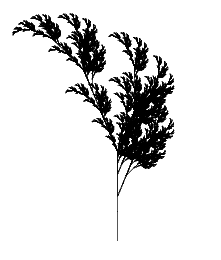
\includegraphics[width=\textwidth]{ferns/plant1.png}
    \caption{(a) $t = 8$, $\delta = 22.5 ^{\circ}$ \\ $\omega: G$ \\ $G \rightarrow F+[[G]-G]-F[-FG]+G$ \\ $F \rightarrow FF$}
	\end{center}
	\end{subfigure}
\hfill
	\begin{subfigure}[tbh]{0.3\textwidth}
	\begin{center}
	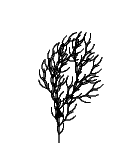
\includegraphics[width=\textwidth]{ferns/plant2.png}
	\caption{(a) $t = 4$, $delta = 22.5^{\circ}$ \\ $\omega: F$ \\ $F \rightarrow FF+[+F-F-F]-[-F+F+F]$}
	\end{center}
	\end{subfigure}
\hfill
	\begin{subfigure}[tbh]{0.3\textwidth}
	\begin{center}
	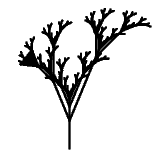
\includegraphics[width=\textwidth]{ferns/plant3.png}
	\caption{(a) $t = 6$, $\delta = 22.5^{\circ}$ \\ $\omega: G$ \\ $G\rightarrow F+[+FFG][G]-FG$ \\ $F \rightarrow FF$}
	\end{center}
	\end{subfigure}
\hfill
	\begin{subfigure}[tbh]{0.3\textwidth}
	\begin{center}
	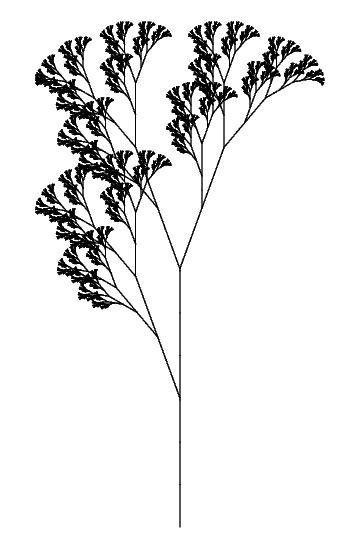
\includegraphics[width=\textwidth]{ferns/plant4.png}
	\caption{(a) $t = 9$, $\delta = 20^{\circ}$ \\ $\omega: G$ \\ $G\rightarrow F[-G]F[+G]-G$ \\ $F \rightarrow FF$}
	\end{center}
	\end{subfigure}
\hfill
	\begin{subfigure}[tbh]{0.3\textwidth}
	\begin{center}
	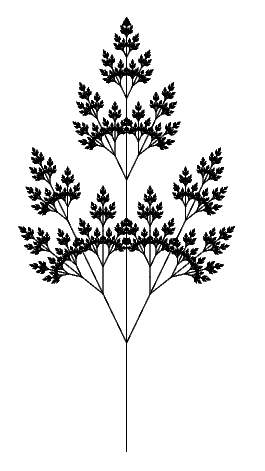
\includegraphics[width=\textwidth]{ferns/plant5.png}
	\caption{(a) $t = 9$, $\delta = 25.7^{\circ}$ \\ $\omega: G$ \\ $G\rightarrow F[-G][+G]FG $\\ $F \rightarrow FF$}
	\end{center}
	\end{subfigure}
\hfill
	\begin{subfigure}[tbh]{0.3\textwidth}
	\begin{center}
	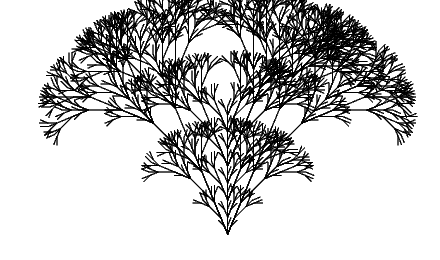
\includegraphics[width=\textwidth]{ferns/plant6.png}
	\caption{(a) $t = 5$, $\delta = 22.5^{\circ}$ \\ $\omega: G$ \\ $G\rightarrow FG[-F[G]-G][G+G][+F[G]+G]$ \\ $F \rightarrow FF$}
	\end{center}
	\end{subfigure}
\hfill
\end{center}
\caption{ Plants from "Fundamentals of Natural Computing}
\end{figure} \label{bookPlants}

\begin{figure}[tbh]
\begin{center}
	\begin{subfigure}[tbh]{0.23\textwidth}
	\begin{center}
	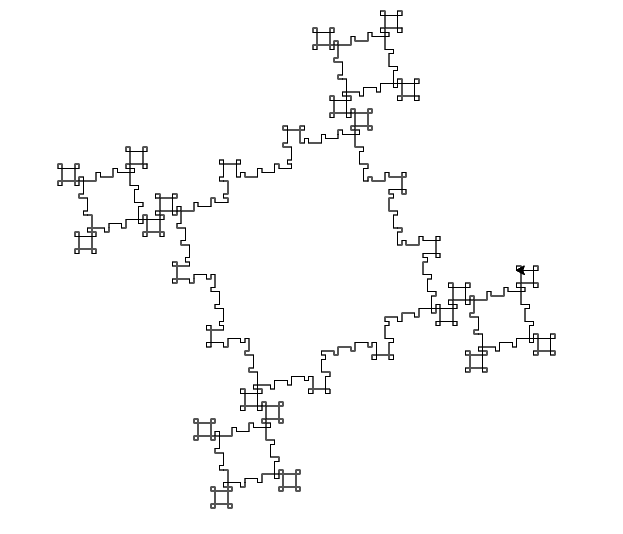
\includegraphics[width=\textwidth]{ferns/my-plant1.png}
	\caption{(a) $t = 4$, $\delta = 90^{\circ}$ \\ $\omega: F+F+F+F$ \\ $F \rightarrow F+F+F-FFF-F$}
	\end{center}
	\end{subfigure}
\hfill
	\begin{subfigure}[tbh]{0.23\textwidth}
	\begin{center}
	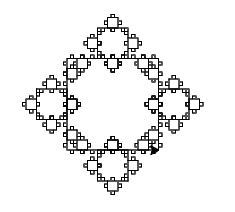
\includegraphics[width=\textwidth]{ferns/my-plant2.png}
	\caption{(a) $t = 4$, $\delta = 90^{\circ}$ \\ $\omega: F+F+F+F$ \\ $F \rightarrow FF+F+F+F+FF$}
	\end{center}
	\end{subfigure}
\hfill
	\begin{subfigure}[tbh]{0.23\textwidth}
	\begin{center}
	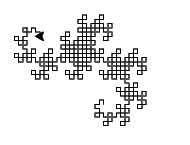
\includegraphics[width=\textwidth]{ferns/my-plant3.png}
	\caption{(a) $t = 4$, $\delta = 90^{\circ}$ \\ $\omega: F-G$ \\ $G \rightarrow F+G $\\ $F \rightarrow F-G$}
	\end{center}
	\end{subfigure}
\hfill
	\begin{subfigure}[tbh]{0.23\textwidth}
	\begin{center}
	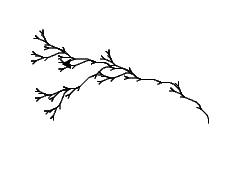
\includegraphics[width=\textwidth]{ferns/my-plant4.png}
	\caption{(a) $t = 4$, $\delta = 22.5^{\circ}$ \\ $\omega: G$ \\ $G \rightarrow FG[-G+]+[G+]F$\\ $F \rightarrow F-G$}
	\end{center}
	\end{subfigure}
\hfill
	\begin{subfigure}[tbh]{0.23\textwidth}
	\begin{center}
	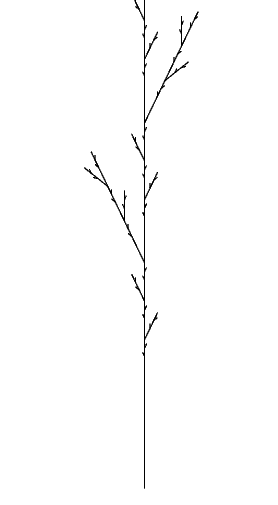
\includegraphics[width=\textwidth]{ferns/my-plant5.png}
	\caption{(a) $t = 4$, $\delta = 25.7^{\circ}$ \\ $\omega: G $\\ $G \rightarrow FFG[-G]FG[+G]FG$\\ $F \rightarrow FF$}
	\end{center}
	\end{subfigure}
\hfill
	\begin{subfigure}[tbh]{0.23\textwidth}
	\begin{center}
	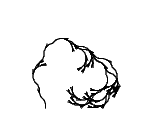
\includegraphics[width=\textwidth]{ferns/my-plant6.png}
	\caption{(a) $t = 4$, $\delta = 22.5^{\circ}$ \\ $\omega: G $\\ $G \rightarrow F+G+[-G-]-[+G+]+F$\\ $F \rightarrow F-G$}
	\end{center}
	\end{subfigure}
\hfill
	\begin{subfigure}[tbh]{0.23\textwidth}
	\begin{center}
	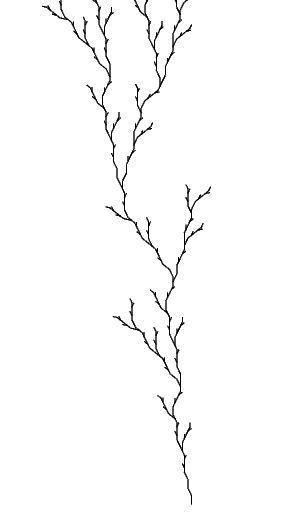
\includegraphics[width=\textwidth]{ferns/my-plant7.png}
	\caption{(a) $t = 4$, $\delta = 25.7^{\circ}$ \\ $\omega: G$ \\ $G \rightarrow FF+G[-G]FG[+G]F-G$\\ $F \rightarrow FF$}
	\end{center}
	\end{subfigure}
\hfill
	\begin{subfigure}[tbh]{0.23\textwidth}
	\begin{center}
	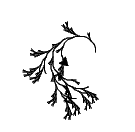
\includegraphics[width=\textwidth]{ferns/my-plant8.png}
	\caption{(a) $t = 4$, $\delta = 22.5^{\circ}$ \\ $\omega: G$ \\ $G \rightarrow F[+G+[-G-]-[+G+]+]F$\\ $F \rightarrow F-G$}
	\end{center}
	\end{subfigure}
\hfill
	\begin{subfigure}[tbh]{0.23\textwidth}
	\begin{center}
	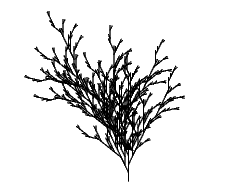
\includegraphics[width=\textwidth]{ferns/my-plant9.png}
	\caption{(a) $t = 4$, $\delta = 22.5^{\circ}$ \\ $\omega: G$ \\ $G \rightarrow FG[-G+]-[G+]F$\\ $F \rightarrow F+G$}
	\end{center}
	\end{subfigure}
\hfill
	\begin{subfigure}[tbh]{0.23\textwidth}
	\begin{center}
	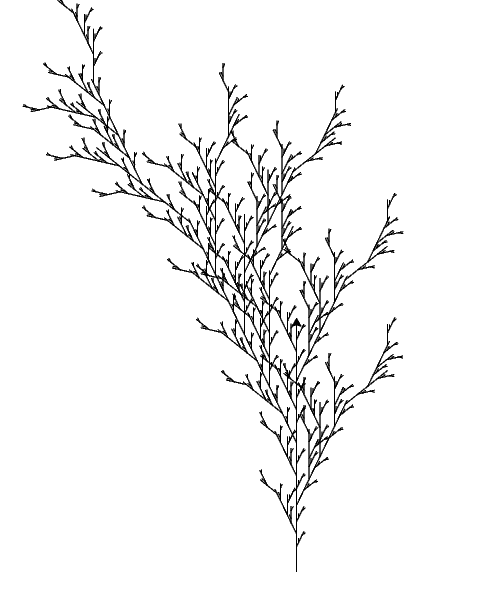
\includegraphics[width=\textwidth]{ferns/my-plant10.png}
	\caption{(a) $t = 4$, $\delta = 25.7^{\circ}$ \\ $\omega: G$ \\ $G \rightarrow FGF[+G[-G]FG[+G]F-]GF+[G+]F$\\ $F \rightarrow FF$}
	\end{center}
	\end{subfigure}
\hfill
\end{center}
\caption{ Plants from "Fundamentals of Natural Computing}
\end{figure} \label{myPlants}

\section{Problem 15}
\textbf{ Implement a RIFS to generate all the fractals whose codes are presented in Table: ~\ref{table:RIFS} } \\
\newline
RIFS is an acronym for Random Iterated Function System (RIFS). An iterated function system (IFS) recursively applies a set of affine transformations to each point in a point list. Generally, the affine transformations are a contractive mapping.  Unless you are zooming in, there is a depth at which the points are very dense and not all of them need to be mapped. This is where the RIFS comes into play. Each point in the point list has one of the functions of the set applied to it. The resolution is still good and the program runs much faster because there are few computations done. 

The codes (functions) given in ~\ref{table:RIFS} are defined such that \textit{w} is the function number, \textit{a, b, c, d} are scaling factors, \textit{e, f} are offset values and \textit{p} is the probability the function will be selected. These values are used in the equation for affine transformation ~\ref{affine_transformation}. The Sierpinski Gasket and Square fractals must have an initial point list to perform the transformations. The Barnsley Fern and Tree need only a single point to perform the transformations. Figure ~\ref{fractals} shows the Sierpinski Gasket, Square, Bransley Fern and Tree generated using the RIFS codes. 

\begin{equation}
w(x_1 , x_2) = ( a x_1 + b x_2 + e, c x_1 + d x_2 + f )
\end{equation} \label{affine_transformation}

\begin{figure}[tbh]
\begin{center}
	\begin{subfigure}[tbh]{0.475\textwidth}
	\begin{center}
	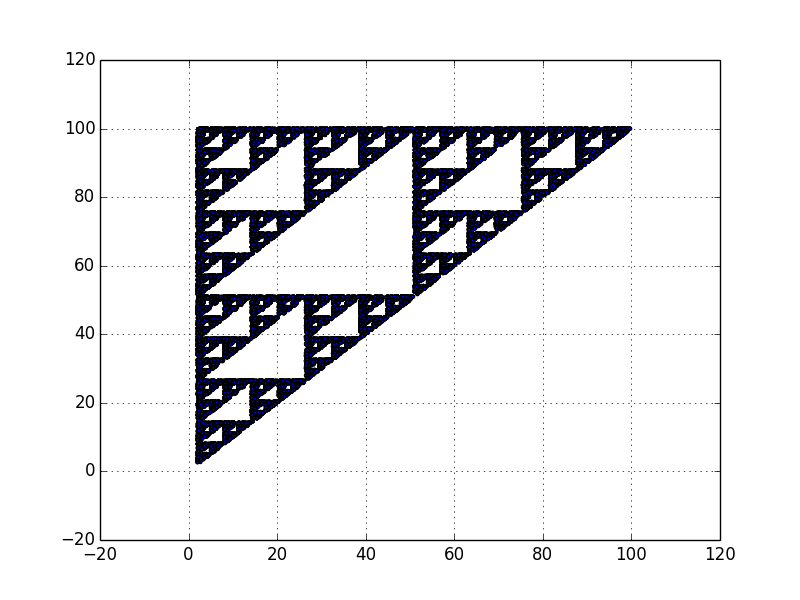
\includegraphics[width=\textwidth]{fractals/SierpinskiGasket.png}
	\caption{ Sierpinski Gasket }
	\end{center}
	\end{subfigure}
\hfill
	\begin{subfigure}[tbh]{0.475\textwidth}
	\begin{center}
	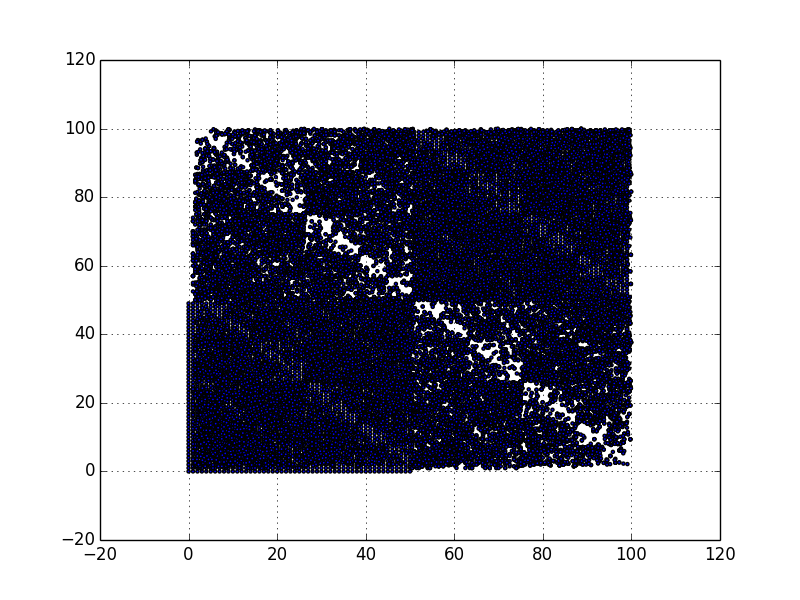
\includegraphics[width=\textwidth]{fractals/Square.png}
	\caption{ Square }
	\end{center}
	\end{subfigure}
\hfill
	\begin{subfigure}[tbh]{0.475\textwidth}
	\begin{center}
	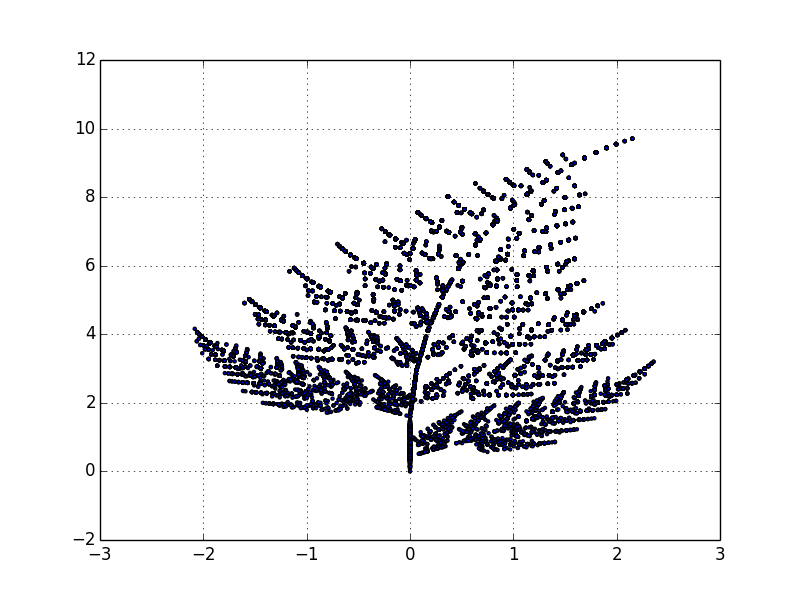
\includegraphics[width=\textwidth]{fractals/BarnsleyFern.png}
	\caption{ Barnsley Fern }
	\end{center}
	\end{subfigure}
\hfill
	\begin{subfigure}[tbh]{0.475\textwidth}
	\begin{center}
	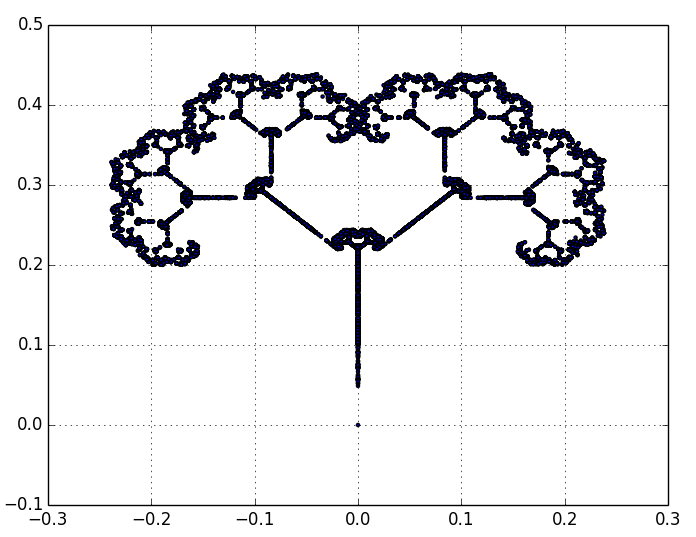
\includegraphics[width=\textwidth]{fractals/Tree.png}
	\caption{ Tree }
	\end{center}
	\end{subfigure}
\hfill

\end{center}
\caption{Plots of Various Fractals \label{fractals} }
\end{figure}

\begin{table}[ht]
\caption{RIFS codes to generate fractals} 
	\subcaption{Sierpinski Gasket}
	\centering 
	\begin{tabular}{c c c c c c c c} 
	\hline\hline 
	w & a & b & c & d & e & f & p\\ [0.5ex] 
	\hline 
	1 & 0.5 & 0 & 0 & 0.5 & 1 & 1 & 0.33 \\
	2 & 0.5 & 0 & 0 & 0.5 & 1 & 50 & 0.33\\
	3 & 0.5 & 0 & 0 & 0.5 & 50 & 50 & 0.34 \\
	\hline 
\end{tabular}
\bigskip
	\subcaption{ Square }
	\centering 
	\begin{tabular}{c c c c c c c c} 
	\hline\hline 
	w & a & b & c & d & e & f & p\\ [0.5ex] 
	\hline 
	1 & 0.5 & 0 & 0 & 0.5 & 1 & 1 & 0.25\\
	2 & 0.5 & 0 & 0 & 0.5 & 50 & 1 & 0.25\\
	3 & 0.5 & 0 & 0 & 0.5 & 1 & 50 & 0.25\\
	4 & 0.5 & 0 & 0 & 0.5 & 50 & 50 & 0.25\\
	\hline 
\end{tabular}
\bigskip
	\subcaption{ Barnsley Fern }
	\centering 
	\begin{tabular}{c c c c c c c c} 
	\hline\hline 
	w & a & b & c & d & e & f & p\\ [0.5ex] 
	\hline 
	1 & 0 & 0 & 0 & 0.16 & 0 & 0 & 0.01 \\
	2 & 0.85 & 0.04 & -0.04 & 0.85 & 0 & 1.6 & 0.85\\
	3 & 0.2 & -0.26 & 0.23 & 0.22 & 0 & 1.6 & 0.07 \\
	4 & -0.15 & 0.28 & 0.26 & 0.24 & 0 & 0.44 & 0.07 \\
	\hline 
\end{tabular}
\bigskip
	\subcaption{ Tree }
	\centering 
	\begin{tabular}{c c c c c c c c} 
	\hline\hline 
	w & a & b & c & d & e & f & p\\ [0.5ex] 
	\hline 
	1 & 0 & 0 & 0 & 0.5 & 0 & 0 & 0.05 \\
	2 & 0.42 & -0.42 & 0.42 & 0.42 & 0 & 0.2 & 0.40\\
	3 & 0.42 & 0.42 & -0.42 & 0.42 & 0 & 0.2 & 0.40\\
	4 & 0.1 & 0 & 0 & 0.1 & 0 & 0.2 & 0.15 \\
	\hline 
\end{tabular}
\end{table} \label{table:RIFS}


\section{ Problem 21 }
\textbf{ Implement the random midpoint displacement algorithm in 3D and generate some fractal landscapes. Study the influence of \textit{H} on the landscapes generated. } \\
\newline

In 2D, the random midpoint displacement starts with a line, determines the midpoint and randomly perturbs it using equations ~\ref{midpointDisplacement} and ~\ref{roughness}. In equation ~\ref{roughness}, $\Delta(i)$ stores the value for depth $i$, $\sigma$ is the standard deviation of the Gaussian distribution, $H$ is the `roughness factor'. $H$ is always $ 0 < H < 1$. The closer to 0, the more rough the surface will be. The closer to 1, the more smooth the surface will be.  In equation ~\ref{midpointDisplacement} $x_1$ is the new value for the midpoint, $x_0$ is the left end point, $x_2$ is the right end point, $\Delta(t)$ is  from equation ~\ref{roughness}, $t$ is the recursion depth and $rand$ is a random number. Now, there are two line segments and the midpoint of each line segment is perturbed. This method is recursively applied while decreasing the perturbation amount for each depth. 

\begin{equation}
x_1 = 0.5 ( x_0 + x_2 ) + \Delta(t)  rand
\end{equation} \label{midpointDisplacement}

\begin{equation}
\Delta(i) = \sigma (H)^{(i+1)/2)}
\end{equation} \label{roughness}

The random midpoint displacement for 3D starts with a 2D box. The box is subdivided using the midpoints of the edges, so one box becomes four boxes, four boxes becomes sixteen, ect. The intersections of the midpoint lines becomes the perturbation points. They are perturbed in the same manner as the 2D method except the average is the average of the four surrounding points. Figure ~\ref{surfaces} shows some surfaces with varying $H$ values.


\begin{figure}[tbh]
\begin{center}
	\begin{subfigure}[tbh]{0.475\textwidth}
	\begin{center}
	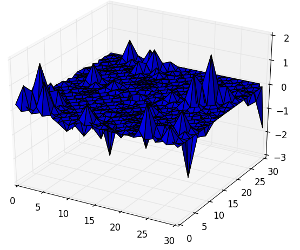
\includegraphics[width=\textwidth]{fractals/brownianSurface_s1-5_H0-2.png}
	\caption{ $\sigma = 1.5$, $H = 0.2$ }
	\end{center}
	\end{subfigure}
\hfill
	\begin{subfigure}[tbh]{0.475\textwidth}
	\begin{center}
	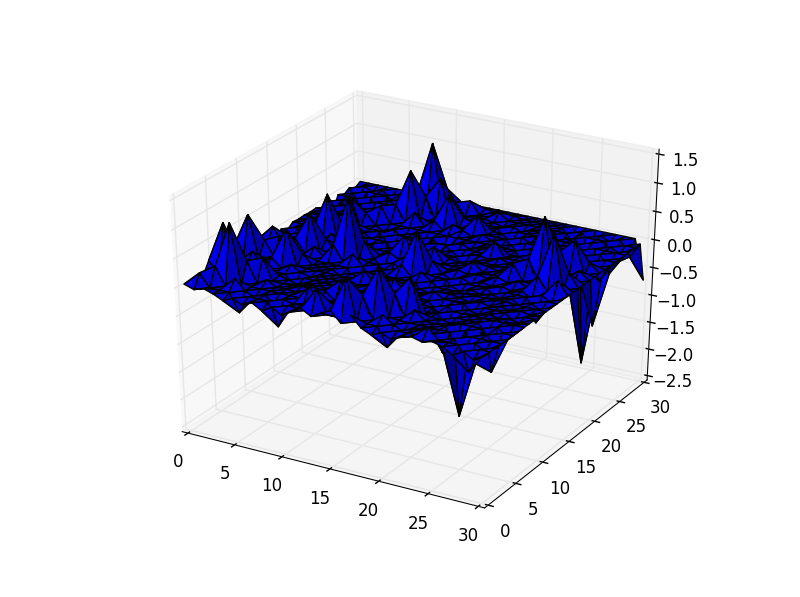
\includegraphics[width=\textwidth]{fractals/brownianSurface_s1-5_H0-5.png}
	\caption{$\sigma = 1.5$, $H = 0.5$}
	\end{center}
	\end{subfigure}
\hfill
	\begin{subfigure}[tbh]{0.475\textwidth}
	\begin{center}
	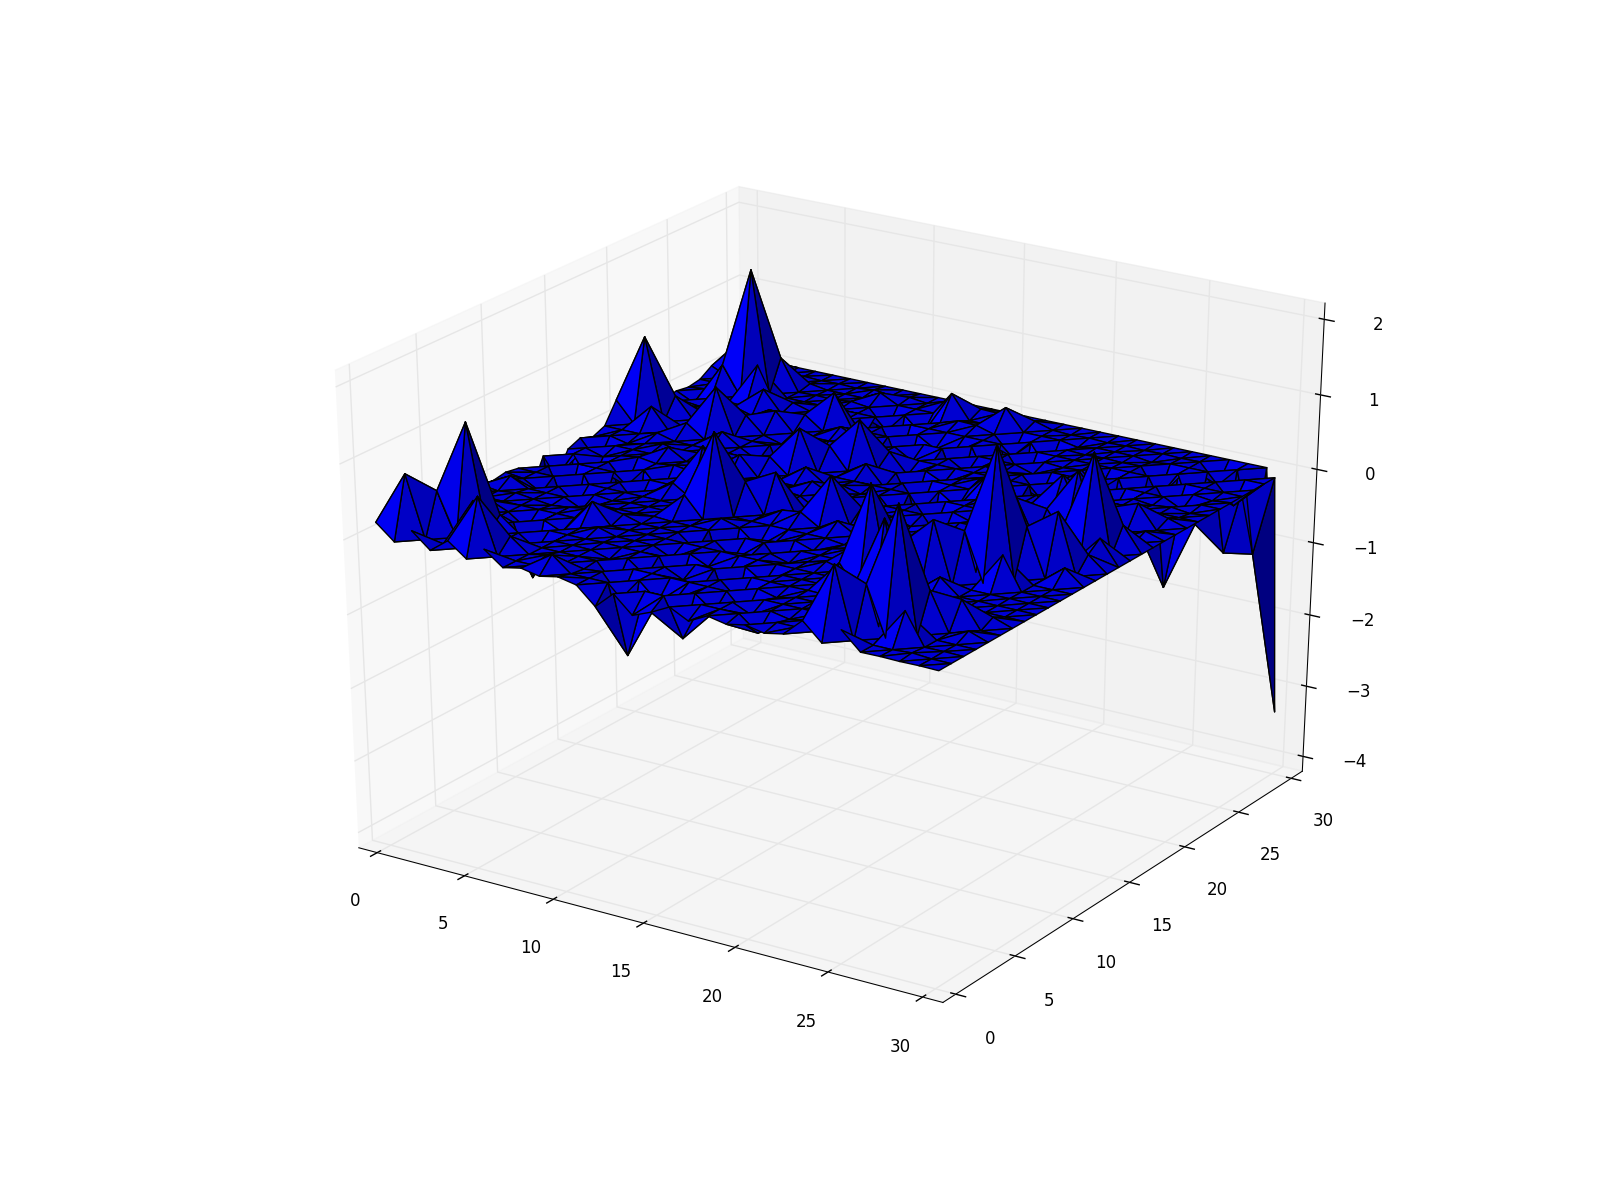
\includegraphics[width=\textwidth]{fractals/brownianSurface_s1-5_H0-75.png}
	\caption{ $\sigma = 1.5$, $H = 0.75$ }
	\end{center}
	\end{subfigure}
\hfill
	\begin{subfigure}[tbh]{0.475\textwidth}
	\begin{center}
	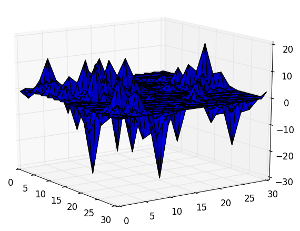
\includegraphics[width=\textwidth]{fractals/brownianSurface_s5_H0-75.png}
	\caption{ $\sigma = 5$, $H = 0.75$ }
	\end{center}
	\end{subfigure}
\hfill

\end{center}
\caption{Brownian Surfaces with Varying $\sigma$'s and $H$'s \label{surfaces} }
\end{figure}
